\documentclass[12pt]{article}

\usepackage[utf8]{inputenc}
\usepackage[T1]{fontenc}
\usepackage[english]{babel}
\usepackage{graphicx}
%\usepackage{amsthm}
\usepackage{amsmath}
\usepackage{fullpage}
\usepackage{amssymb}
\usepackage{mathrsfs}
\usepackage{array}
\usepackage{colortbl}
\usepackage{siunitx}
\usepackage{mathtools}
\usepackage[colorinlistoftodos]{todonotes}
\usepackage{subcaption}
\usepackage{float}
\usepackage{url}
\usepackage{amsmath}
\usepackage{gensymb}
\usepackage{hyperref}
\usepackage{wasysym}
\usepackage{listings} 
\usepackage{subfig}
\usepackage{breqn}
\usepackage{eqnarray}
\usepackage{natbib}
\usepackage{rotating}
%\usepackage[top=1.0in, bottom=1.0in, left=1.0in, right=1.0in]{geometry}

\DeclareFixedFont{\ttb}{T1}{txtt}{bx}{n}{12} % for bold
\DeclareFixedFont{\ttm}{T1}{txtt}{m}{n}{12}  % for normal

\usepackage{color}
\definecolor{deepblue}{rgb}{0,0,0.5}
\definecolor{deepred}{rgb}{0.6,0,0}
\definecolor{deepgreen}{rgb}{0,0.5,0}

% Python style for highlighting
\newcommand\pythonstyle{\lstset{
language=Python,
basicstyle=\ttm,
otherkeywords={self},             % Add keywords here
keywordstyle=\ttb\color{deepblue},
emph={MyClass,__init__},          % Custom highlighting
emphstyle=\ttb\color{deepred},    % Custom highlighting style
stringstyle=\color{deepgreen},
frame=tb,                         % Any extra options here
showstringspaces=false            %
}}


\lstset{
  basicstyle=\ttfamily,
  columns=fullflexible,
  breaklines=true,
  postbreak=\mbox{\textcolor{red}{$\hookrightarrow$}\space},
}

% Python environment
\lstnewenvironment{python}[1][]
{
\pythonstyle
\lstset{#1}
}
{}

% Python for external files
\newcommand\pythonexternal[2][]{{
\pythonstyle
\lstinputlisting[#1]{#2}}}

% Python for inline
\newcommand\pythoninline[1]{{\pythonstyle\lstinline!#1!}}

\title{sloan.tex}

\begin{document}

	\newcommand{\HRule}{\rule{\linewidth}{0.5mm}}

\begin{titlepage}
\begin{center}




\vspace*{2.5cm}



\includegraphics[width=0.4\textwidth]{EPFL-Logo-CMJN.eps}\\[1.5cm]


\textsc{\LARGE Space Technologies Minor Project}\\[1.5cm]


\HRule \\[0.4cm]
{ \huge \bfseries Collision-free positioning of optical fibers: \\ from MOONS to Sloan \\[0.4cm] }

\HRule \\[1.5cm]

{\Large 
Author : Clément \textsc{Camus}

\vspace*{0.8cm}

Supervisors : Denis \textsc{Gillet} \& Jean-Paul \textsc{Kneib}}
\vfill


{\large \today}

\end{center}
\end{titlepage}
	\clearpage
	
	\tableofcontents
	\clearpage

	\section{Introduction} \label{introduction}

The purpose of this project is the transfer of knowledge and technology from the MOONS trajectory computation and collision avoidance software, made by Dr. Laleh Makarem \cite{makarem_a, makarem_b, makarem_c} \& Dominique Tao, to the Sloan project, which role will be similar: compute trajectories of hundreds of actuators on a plane, with an hexagonal arrangement, to place fibers under targets, avoiding collision and deadlocks. Therefore, the two main goals are the update of the program for the Sloan case, and the improvement of the convergence rate (that is, the number of actuator able to reach their assigned target without any collision or deadlocks).
\\

During this project, I mainly worked on the first goal. This report aim at explaining the work I have done during this semester, as well as the work still ongoing. To do so, a reminder explaining the differences between the two projects will be given. Then, Sections \ref{circles} and \ref{parameters} will explain the change in the architecture of the software, especially the introduction of a program generating the actuators structures for the Sloan project as well as the centralisation of every parameters in a single text file. Section \ref{set_target} shows the update of the target setting function and the fiber attribution, regarding to the major changes on the Sloan project, being the adding of new fibers on each ferules. In Section \ref{target_generator}, a small script enabling the generation of target files to test the software will be presented. Section \ref{visualisation} shows the improvements implemented on the animation available at the end of the computation. Finally, Sections \ref{to-do} and \ref{conclusion} will describe ongoing jobs as well as the rest of the tasks to be done to obtain a working software for the Sloan project. Changes in the code of the software can be seen in the Appendices.
	\clearpage

	\section{From MOONS to Sloan : Reminder} \label{reminder}

This section aims at explaining the differences between the MOONS project and the Sloan one, to understand the path taken in the rest of the project.
\\

MOONS (Multi-Object Optical and Near-infrared Spectrograph) is a design for the Very Large Telescope, the European Southern Observatory telescope facility. The fiber system is made of 1'000 actuators whose role is to position fibers on the surface of the telescope. Each actuator has two degrees of freedom as shown on Figure \ref{fig:reminder:actuator}. At the end of the second arm, each ferule contained only one near-IR fiber. The actuator structure had an hexagonal shape, with several holes for camera and fiducial tools.
\\

\begin{figure}[h]
\begin{center}
	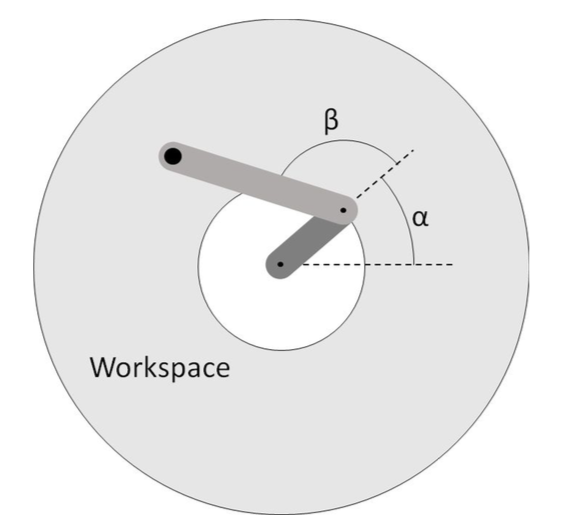
\includegraphics[width=0.40\textwidth]{reminder/actuator.png}
	\caption{Actuator's design, with the two degrees of freedom being $\alpha$ and $\beta$ angles. The arm displaced on the $\alpha$ angle is the $\alpha$-arm, while the arm displaced on the $\beta$ angle is the $\beta$-arm. The black dot at the end of the $\beta$-arm is the ferule, containing two to three fibers.}
	\label{fig:reminder:actuator}
\end{center}
\end{figure}

\begin{figure}[h]
\begin{center}
	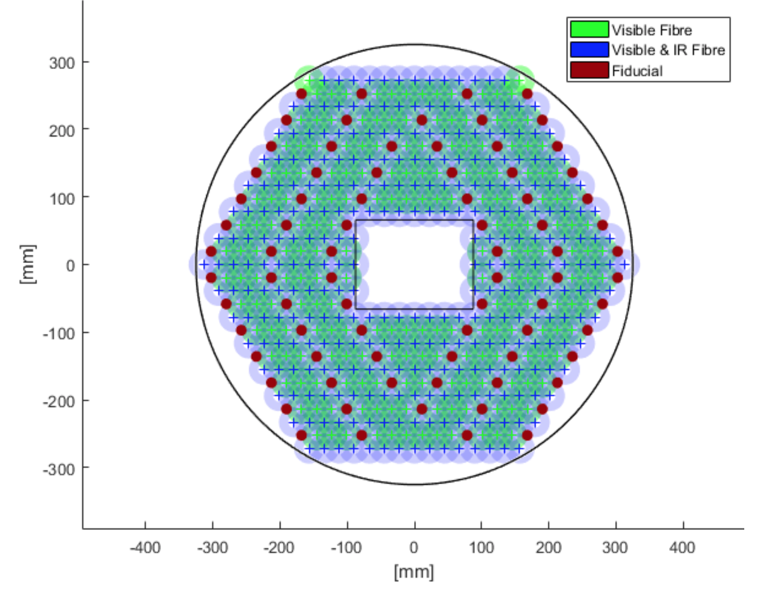
\includegraphics[width=\textwidth]{reminder/sloan_arrangement.png}
	\caption{Actuators structure for the Sloan project.}
	\label{fig:reminder:sloan_arrangement}
\end{center}
\end{figure}

\begin{figure}[h]
\begin{center}
	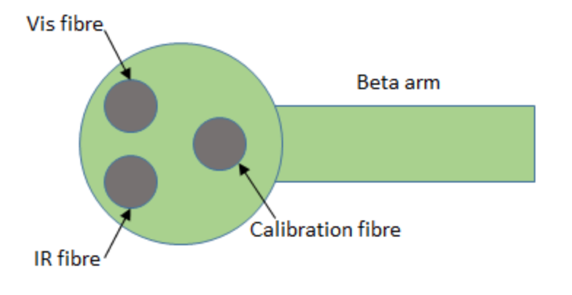
\includegraphics[width=0.40\textwidth]{reminder/ferule.png}
	\caption{Ferule design for the Sloan project.}
	\label{fig:reminder:ferule}
\end{center}
\end{figure}


For the Sloan telescope, the arrangement, as seen on Figure \ref{fig:reminder:sloan_arrangement}, is also hexagonal. However, the system is made of 500 actuators, with a rectangle in the middle of the telescope. Some actuator slots are taken by fiducial tools, in red on Figure \ref{fig:reminder:sloan_arrangement}.\\

The main update from the Sloan system is the presence of two to three fibers on each ferule. As shown on Figure \ref{fig:reminder:sloan_arrangement}, each ferule contains both a visible and a calibration fiber, while 300 of the 500 motors contain an additional IR fiber. This structure allows a spatial coverage by IR fibers of 99.5\% of the surface reachable by actuators, even if IR fibers are present only on three fifth of the actuators. A scheme of the new ferule is shown on Figure \ref{fig:reminder:ferule}.


	\clearpage
	
	\section{Sloan actuator structure} \label{circles}

As said in Section \ref{reminder}, the Sloan telescope arrangement is made of 500 actuators, in an hexagonal shape. In the MOONS project, actuators types and position were listed in a cfg file. For time and practical reasons, this has been changed. A program called "circles.py" has been created to contain all actuators position and properties. The program is launched at each software's run, ensuring that, if a structure's parameter is changed (space between two parameters, fiber properties of several actuators etc.), the program will be automatically updated.

\begin{figure}[h]
\begin{center}
	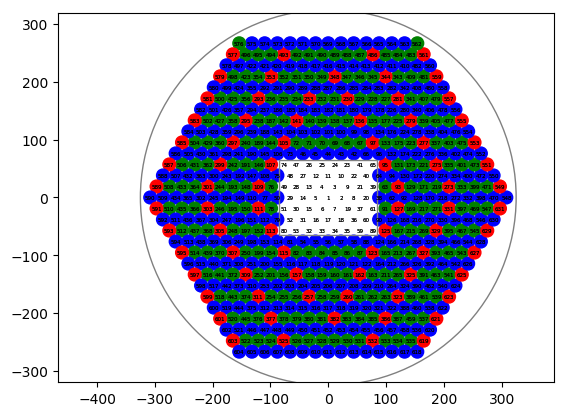
\includegraphics[width=\textwidth]{circles/sloan_arrangement.png}
	\caption{Actuators structure for the Sloan project.}
	\label{fig:sloan:arrangement}
\end{center}
\end{figure}

The script creates the structure shown on Figure \ref{fig:sloan:arrangement}. One can compare it with the structure desired shown on Figure \ref{fig:reminder:sloan_arrangement}. The creation and indexation of actuators work as follow :

\begin{enumerate}
	\item A first actuator is created on position (0, 0).
	\item Then, using several functions available in the Appendix 1, a layer made of 6 actuators is created, beginning by the one on the right of the first actuator (actuator 2). The second function creates an actuator (actuator 3) on the top left of the preceding actuator, the third function creates an actuator (actuator 4) on the left of actuator 3 and so on. As the first layer is made of 6 actuators, each function is applied once.
	\item The second layer, made of 12 actuators, is made by applying the first function to create actuator 8. Then the second function is applied two times, creating actuators 9 and 10, and so on until the layer is finished.
	\item The rest of the structure is made by applying Step 3 until a certain quantity of actuator has been created.
\end{enumerate} 

The indexation and construction of the structure is illustrated in the Appendix 1.
\\

 Then, the second part of the program classifies each actuator in one of the four following categories: empty, fiducial, IR or visible. Each actuator positioned in the rectangle in the middle of the telescope is set in the Empty category. Each actuator positioned on a fiducial slot as shown on Figure \ref{fig:sloan:arrangement} is set in the Fiducial category. As shown on Figure \ref{fig:sloan:arrangement}, every actuator containing an IR fibre have similar y-coordinates, which is a certain real number times any discrete (positive, negative or null) number; any actuator which is not an Empty or a Fiducial having the aforementioned y-coordinate property is set as IR. Any other actuator, plus the two actuators on the top left and top right of the arrangement (see Figure \ref{fig:sloan:arrangement}) are set as Visible.
\\

The script works for the structure set on December 2017. It is still possible to modify it easily; for instance :

\begin{itemize}
	\item If the middle rectangle size is increased (or decreased), the only update to make is the addition (or subtraction) of actuator's indexes in the text file "empty.txt".
	\item If some actuators will be replaced by fiducial (or some fiducial removed), the only update is the addition (or subtraction) of actuator's indexes in the text file "fiducial.txt".
	\item If the dimensions of the structure are changed (space between actuators), the program updates automatically the list of actuators set as IR.
	\item If new actuators have to be added on the limits of the existing ones to approach the circular shape, only two steps are required: adding new actuator layers, and adding a new requirement such as the radial coordinate of the actuator has to be inferior to the radius of the telescope (or manually classifying the actuators created outside of the focal plane as Empty).
\end{itemize}

An example of each one of those adjustment is shown on Figure \ref{fig:sloan:examples}.

\begin{figure}[h]
	\begin{center}
		\begin{subfigure}{0.85\textwidth}
			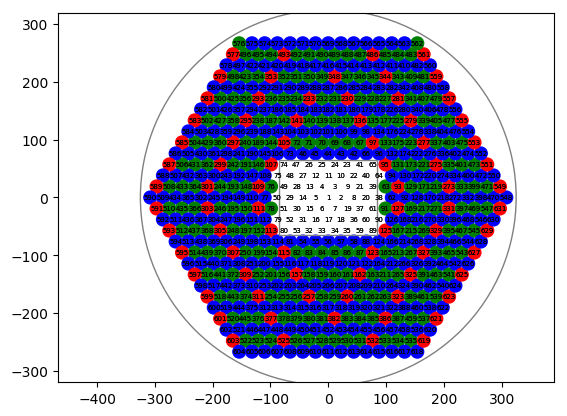
\includegraphics[width=\textwidth]{circles/sloan_adding_empty.png}
			\caption{}
		\end{subfigure}

		\begin{subfigure}{0.85\textwidth}
			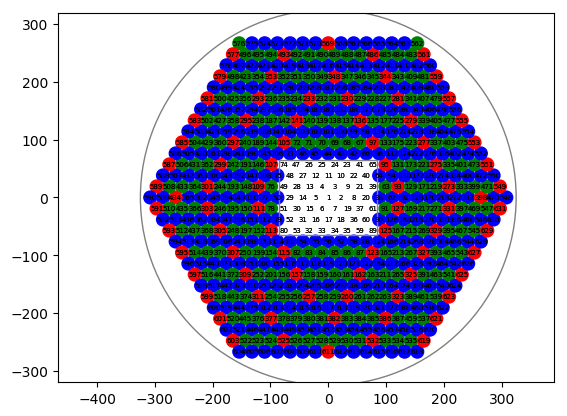
\includegraphics[width=\textwidth]{circles/sloan_adding_fiducial.png}
			\caption{}
		\end{subfigure}
	\end{center}
\end{figure}
		
\begin{figure}[h]\ContinuedFloat
\begin{center}
		\begin{subfigure}{0.85\textwidth}
			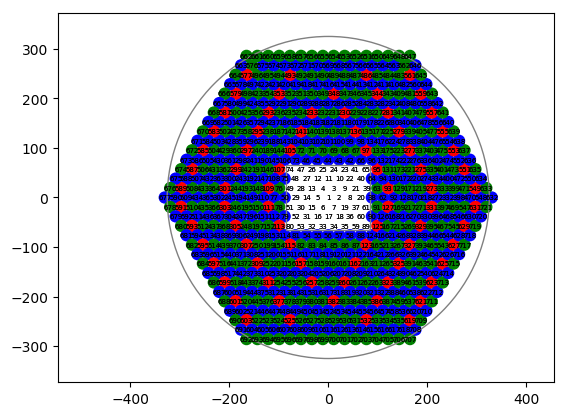
\includegraphics[width=\textwidth]{circles/sloan_adding_layer.png}
			\caption{}
		\end{subfigure}
		
		\begin{subfigure}{0.85\textwidth}
			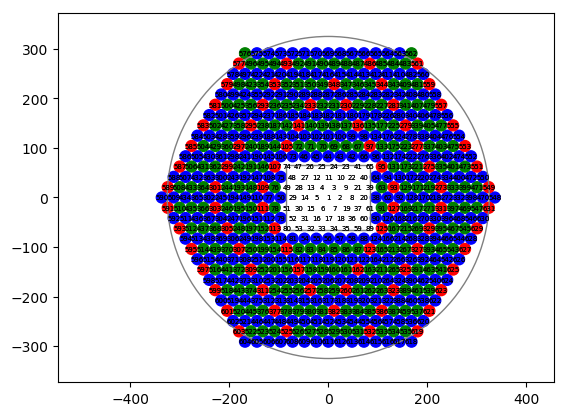
\includegraphics[width=\textwidth]{circles/sloan_adding_separation.png}
			\caption{}
		\end{subfigure}
		\caption{Examples of adjustments made on the actuator's structure only by modifying text files. (a) Addition of six indexes (38, 50, 64, 75, 79, 90) in the file empty.txt. (b) Addition of four indexes (398, 434, 569, 611) in the file fiducial.txt. (c) Addition of a layer by modifying an entry in the file parameters.txt. (d) Increase of the separation length between actuators by modifying an entry in the file parameters.txt.}
		\label{fig:sloan:examples}
	\end{center}
\end{figure}
	\clearpage
	
	\section{Parameters}  \label{parameters}

Previously, the constants needed for the program to be launched (telescope's and actuators dimensions, DNF parameters etc.) were scattered all over the software. Thus, any attempt to modify one of those parameter was preceded by a research for the location of the variable definition in one of the programs. For instance, the previous software contained, on three different programs, the codes in Figures  \ref{fig:appendix:parameters_former_fps}, \ref{fig:appendix:parameters_former_pa_dnf} and \ref{fig:appendix:parameters_former_path} in Appendix 2. Moreover, a large part of those parameters were not at the very beginning of each program, but sometimes after the 100th code line, making the research for a variable tedious. \\

To simplify the change of the variables, each one of them have been moved in a text file called "parameters.txt". The program "parameters.py" then looks inside this text file the value of the parameters, and gives those values to the rest of the software. This allows an efficient modification of any parameter and minimises the hardcoding problem.
	\clearpage

	\section{Target assigning function update} \label{set_target}

The target assigning function's purpose ($\textrm{set_target}$ in fps_shared.py) is to propose a target for each actuator. If the target fulfills certain criteria, especially on its position (the actuator must be able to reach the target), then the actuator is assigned to the target. It means the actuator's ferule's center will be moved to the target position.\\

Two updates had to be made: first, the center of the ferule is not anymore the position of the fiber; as shown in Section \ref{reminder} on Figure \ref{fig:reminder:ferule}, the actuator has to be placed under the desired fiber. Furthermore, we have to be able to ask in advance for each target to be seen by a visible fiber, a calibration fiber or an IR fiber. The first problem will be treated in Section \ref{set_target_1}, while the second one will be covered in Section \ref{fiber_attribution}.

\subsection{$\textrm{set_target}$} \label{set_target_1}

As said earlier, the function $\textrm{set_target}$ is used to assign a target to a certain actuator. If the target was it the range of action of the actuator, then the actuator was assigned to this target. Otherwise, the assignment stoped. In addition to assigning the target to the actuator, the function gave the actuator's ferule's center its destination, which was set at the position of the target. As said in the Reminder, the position of the fiber is not anymore at the center of the ferule, but at one of three points near from the ferule, as shown on Figure \ref{fig:reminder:ferule}. This situation imposed two tasks:

\begin{enumerate}
	\item Knowing and setting in advance which fiber the target has to be surveyed with.
	\item Changing the actuator desired position depending on the fiber used.
\end{enumerate}

The first task had been solved the following way: in addition to the position, parity and priority of each target, the target file now requires a new column to be filled with a number (as for the priority) between 1, 0 and -1 depending on the chosen fiber. The correspondance is shown in Table \ref{table:set_target:target_file_fiber}. Former and new target file structures, with two example lines, are shown in Tables \ref{table:set_target:former_target} and \ref{table:set_target:new_target}.
\\

The second tasks required more reasoning. The following ideas were studied:

\begin{enumerate}
	\item Drifting the position of the target depending on the choice of the fiber.
	\item Moving each motors to the target (under the center), and then ask a small displacement to move the fiber under the target.
	\item Changing the coordinates of the wished position for each motor, depending on the wished fiber.
	%\item Relocating the position of the center of the ferule depending on the wished fiber.
\end{enumerate}

The first proposition was removed, as it adds confusion in the software between the real position of the target and the virtual one, besides visualisation problems.\\

The second one was also removed, as it doesn't take into account deadlocked actuators, and can lead to collisions during the part where each actuator move the ferule to the good position. Moreover, the change in the position depends on the actual position of the actuator before the correction. \\

The third proposition has been chosen for its simplicity: after setting the destination for the actuator's ferule's center, a correction is added, in the referential of the actuator, depending on the fiber used. The code added can be seen in the Appendix 3. Notwithstanding, it appears this technique does not work in our case: if the two degrees of freedom available would have been the radius and the angle, the modification of the target's position in the center's ferule's referential would have been unique. However, as we have two angles as degrees of freedom, there exists  an infinite number of combination ($\alpha$, $\beta$) respecting the correction aforementioned: first, there is two set of combination depending on the parity (for a fixed $\alpha$, both $\beta$ and $\frac{\pi}{2}-\beta$ give the same solution), but furthermore, targets randomly generated are generally positioned on spots where the solution couple ($\alpha$, $\beta$) is not unique, but continuous. Hence, the correction to the actuator's position will depends on the final ($\alpha$, $\beta$), coming down to solution 2.

\begin{table}[h]
	\begin{center}
	\begin{tabular}{|c|c|}
	\hline
	Indicator & Fiber used  \\
	\hline
1 & IR \\
0 & Visible \\
-1 & Calibration \\
	\hline
	\end{tabular}
	\caption{Correspondance between the target file filling and the fiber to be used.}
	\label{table:set_target:target_file_fiber}
	\end{center}
\end{table}

\begin{table}[h]
	\begin{tabular}{|c|c|c|c|c|c|c|}
	\hline
	R actuator & $\theta$ actuator & R target & $\theta$ target & Arg 1 parity & Arg 2 parity & Priority \\
	\hline
25.2587	& 30 & 32.6135 & 358.578	 & 0 & 1 & 1 \\
25.2587	& 90 & 25.4647 & 67.2179 & 0 & 1 & 1 \\
	\hline
	\end{tabular}
	\caption{Former target file structure with two lines as example.}
	\label{table:set_target:former_target}
\end{table}

\begin{table}[h]
	\begin{tabular}{|c|c|c|c|c|c|c|c|}
	\hline
	R actuator & $\theta$ actuator & R target & $\theta$ target & Arg 1 parity & Arg 2 parity & Priority & Fiber \\
	\hline
25.2587	& 30 & 32.6135 & 358.578	 & 0 & 1 & 1 & 1 \\
25.2587	& 90 & 25.4647 & 67.2179 & 0	 & 1	 & 1 & -1 \\
	\hline
	\end{tabular}
	\caption{New target file structure with two lines as example.}
	\label{table:set_target:new_target}
\end{table}




\subsection{Fiber attribution} \label{fiber_attribution}

The next task will be to use the information on each actuator from the Sloan structure from Section \ref{circles}. More precisely, the goal will be to give the autorisation to actuators to be set on targets only if they are able to. Thus, the following modifications have been made : 

\begin{itemize}
	\item If an actuator is an Empty one (empty rectangle for Sloan) or a Fiducial one, target is never set ($\textrm{Set_target}$ returns False). 
	\item If the target needs an IR fiber, but the proposed actuator only has visible and calibration, target is not set ($\textrm{Set_target}$ returns False).
	\item If the target needs an IR fiber, and the proposed actuator owns an IR fiber, nothing changes.
	\item If the target needs a visible or a calibration fiber, nothing changes.
\end{itemize}

The code added to ensure it can be seen in the Appendix 3.

	\clearpage
		
	\section{Target File Generator} \label{target_generator}

Once the software is ready, it must be tested on several target files, first to be sure it's working properly, and then to work on the convergence rate's improvement. For this purpose, a program called "target_generator" has been created. It is able to create five types of target distribution : Random, Random with a normal distribution, Focused, Focused with a normal distribution, and Homogeneous. An example of each one of those is available on Figure \ref{fig:target_generator:examples}.
\\

\begin{figure}[h]
	\begin{center}
		\begin{subfigure}{0.32\textwidth}
			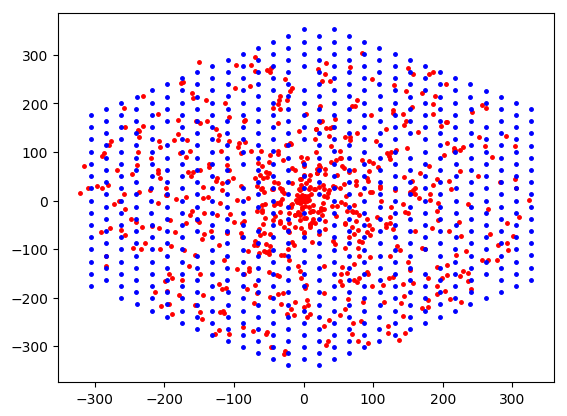
\includegraphics[width=\textwidth]{target/random.png}
			\caption{Example of target file with a random distribution.}
		\end{subfigure}
		\begin{subfigure}{0.32\textwidth}
			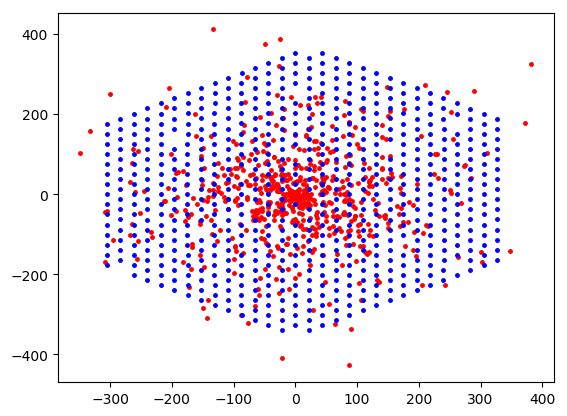
\includegraphics[width=\textwidth]{target/random_normal.png}
			\caption{Example of target file with a random and normal distribution.}
		\end{subfigure}
		\begin{subfigure}{0.32\textwidth}
			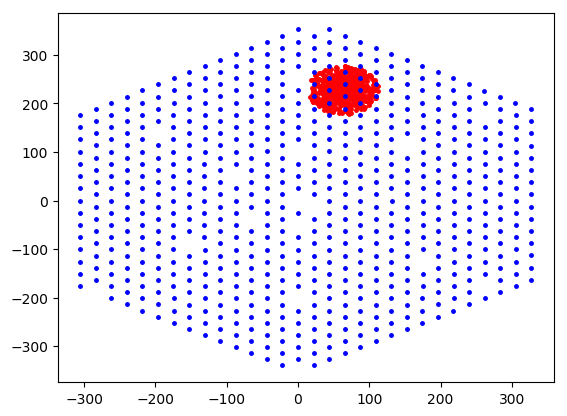
\includegraphics[width=\textwidth]{target/focus.png}
			\caption{Example of target file with a distribution focused on a random point of the telescope.}
		\end{subfigure}
		
		\begin{subfigure}{0.32\textwidth}
			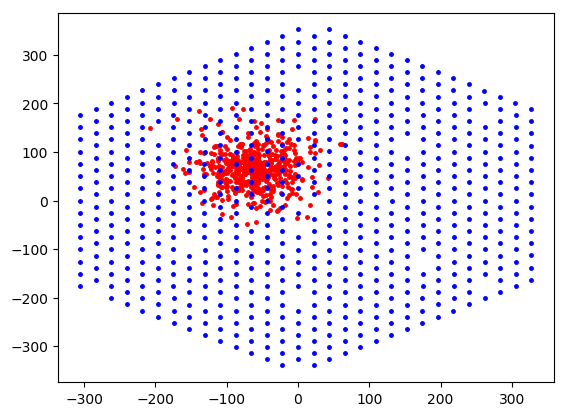
\includegraphics[width=\textwidth]{target/focus_normal.png}
			\caption{Example of target file with a normal distribution focused on a random point of the telescope.}
		\end{subfigure}
		\begin{subfigure}{0.32\textwidth}
			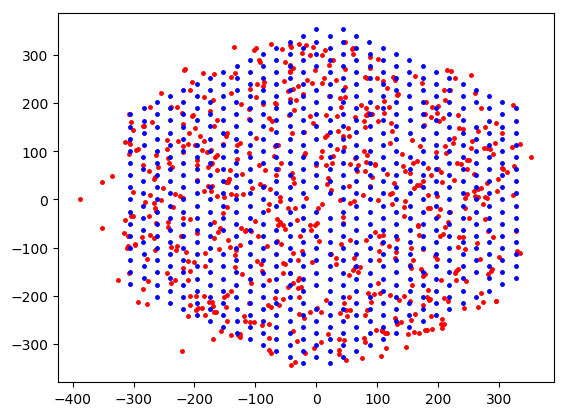
\includegraphics[width=\textwidth]{target/homogeneous.png}
			\caption{Example of target file with an homogeneous distribution.}
		\end{subfigure}
		\caption{Examples of target files generated with the target_generator.py program. Targets are shown in red, while actuators are shown in blue. Actuator positions come from the former software (used for MOONS), and therefore contains its specificity, that is to say some holes where fiducial tools were positioned.}
		\label{fig:target_generator:examples}
	\end{center}
\end{figure}

The homogeneous is the most similar to the MOONS's target files, as it places a target close to each actuators. Therefore, it will also be the one with the highest convergence rate.
	\clearpage
	
	\section{Visualisation} \label{visualisation}

Figure \ref{fig:visualisation} shows two pictures of the the animation available at the end of the computation, for the former and the new software. The improvements are the following: 
\begin{itemize}
	\item The former program only showed the targets surveyed by an actuator. Now, every targets are shown.
	\item As mentioned in Section \ref{fiber_attribution}, each target are set on one of the three fibers available. IR targets are shown in orange, Visible ones in red and Calibration ones in pink. Any target's color change requires hardcoding, however the operation is straightforward; the code to change is given in Appendix 5.
	\item Actuators have also been colorised depending on their functions, respecting the color code on Figures \ref{fig:reminder:sloan_arrangement} and \ref{fig:sloan:arrangement} : empty one are transparent, fiducial ones are red, those with an IR fiber are in blue while the others are in green.
\end{itemize}

\begin{figure}[h]
\begin{center}
	\begin{subfigure}{0.9\textwidth}
		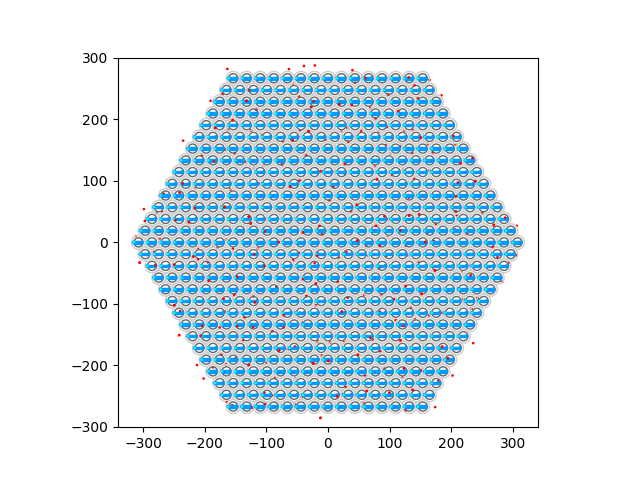
\includegraphics[width=0.9\textwidth]{visualisation/former.png}
		\caption{Former animation picture.}
		\label{fig:visualisation:former}
	\end{subfigure}
	\begin{subfigure}{0.9\textwidth}
		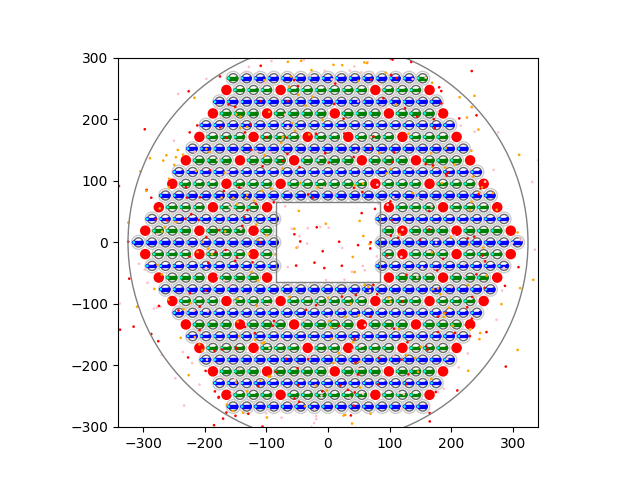
\includegraphics[width=0.9\textwidth]{visualisation/new.png}
		\caption{New animation picture.}
		\label{fig:visualisation:new}
	\end{subfigure}
	\caption{Former and new pictures of the animation available at the end of the computation. Explanations are given in Section \ref{visualisation}.}
	\label{fig:visualisation}
\end{center}
\end{figure}
	\clearpage
	
	\section{To-do list} \label{to-do}

This Section enumerates the remaining main tasks to be done to obtain a working software. \\

The first task to accomplish is, as described in Section \ref{set_target_1}, the correction on the target's position for each actuator depending on the fiber used. This was the main task of this project, however I personally searched in the wrong direction and discovered the mistake too late. \\

Another point to set is on the collision-free update for the Sloan project, especially on the behaviour of fiducial tools on the DNF for its actuator's neighbour. Moreover, the change in the DNF parameters have to be tested so no collision occurs during any process, while verifying that the number of deadlocks stays low.\\ 

Some improvements can me made but are not essential for the operation of the software. Indeed, the convergence rate was still improvable as on the last version. In the same way, the prioritisation can be still improved, to be sure a priority target will be surveyed. \\

The last category of tasks are the improvement of the code in the program: indeed, there is still some feature only used for the MOONS project remaining on the Sloan version. This can slow down the program, lead to mistakes and above all will decrease the understanding of the code.
	\clearpage
	
	\section{Conclusion} \label{conclusion}

The transition from the MOONS software to the Sloan needed two main modifications: the first one was on the structure of the actuators moving on the focal plane, which was different for two projects; the second one concerned the fibers used for the survey, as Sloan's ferules will contain to to three fibers. \\

The first adjustment has been completed so the actuator's structure respects the one discussed on the Preliminary Study Report\cite{study_report}, as shown in Sections \ref{circles} and \ref{visualisation}. Furthermore, the program has been constructed so that some modifications where possible without hardcoding, and so that the program generating the structure also contained informations on the fibers available.\\

The second point has not been completed yet: a solution could not be found yet to correct the target's destination of actuators, so that the desired fiber is positioned under the target surveyed (see Section \ref{set_target}). At least, some possibilities, for instance relocating target's position, could be excluded. The main alternative to work on is asking each actuator to move at the end of the computation to have the fiber on target's position, but it will constitute two challenges, one on the trajectory computation, and another one on the collision-free part of the software. \\

Several components of the software have been improved: the structure has been modified to be able to adjust parameters easily (Section \ref{parameters}), and a new architecture has been designed (see Appendix 4), a program has been created to generate targets file to test the software (Section \ref{target_generator}), and to finish, the visualisation has been modify to take into account the features specific to the Sloan project. \\

I personally enjoyed working on this project, as it was the first time I was working on the development of a software. The software is quite long to understand in depth, so some minor adjustments took some time, but then I could work on python's features I never worked on before (animations, user interface etc.). I would like to thank Prof. Kneib who gave me the opportunity to work on this project, Prof. Gillet for the freedom I had during the semester. 
	\clearpage
	
	\begin{thebibliography}{9}

\bibitem{makarem_a}
   Laleh Makarem,
    \textit{Decentralized multi-robot coordination in crowded workspaces},
	2015.

\bibitem{makarem_b}
	Laleh Makarem, Jean-Paul Kneib, and Denis Gillet,
    \textit{Collision-Free Coordination of Fiber Positioners in Multi-object Spectrographs},
    2015.

\bibitem{makarem_c}
   Laleh Makarem, Jean-Paul Kneib, Denis Gillet, Hannes Bleuler, Mohamed Bouri, Laurent Jenni, Francisco Prada, and Justo Sanchez,
    \textit{Collision avoidance in next-generation fiber positioner robotic systems for large survey spectrographs},
    Astronomy \& Astrophysics,
    2014.

\bibitem{study_report}
	Jean-Paul Kneib, Mohamed Bouri, Denis Gillet, Philipp Horler, Luzius Kronig,
    \textit{SDSS-5 Fibre Positioner Preliminary Study Report, Second Version},
    2017.

\end{thebibliography}
	\clearpage
	
	%Appendix

	\section{Appendix 1: Sloan actuators structure}

\begin{figure}[h]
\begin{center}
	\begin{subfigure}{0.22\textwidth}
	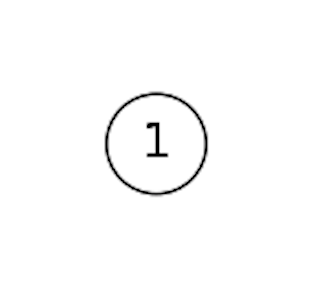
\includegraphics[width=\textwidth]{circles/initialisation}
	\caption{Initialisation.}
	\label{fig:appendix:sloan_structure:initialization}
	\end{subfigure}
	\begin{subfigure}{0.54\textwidth}
	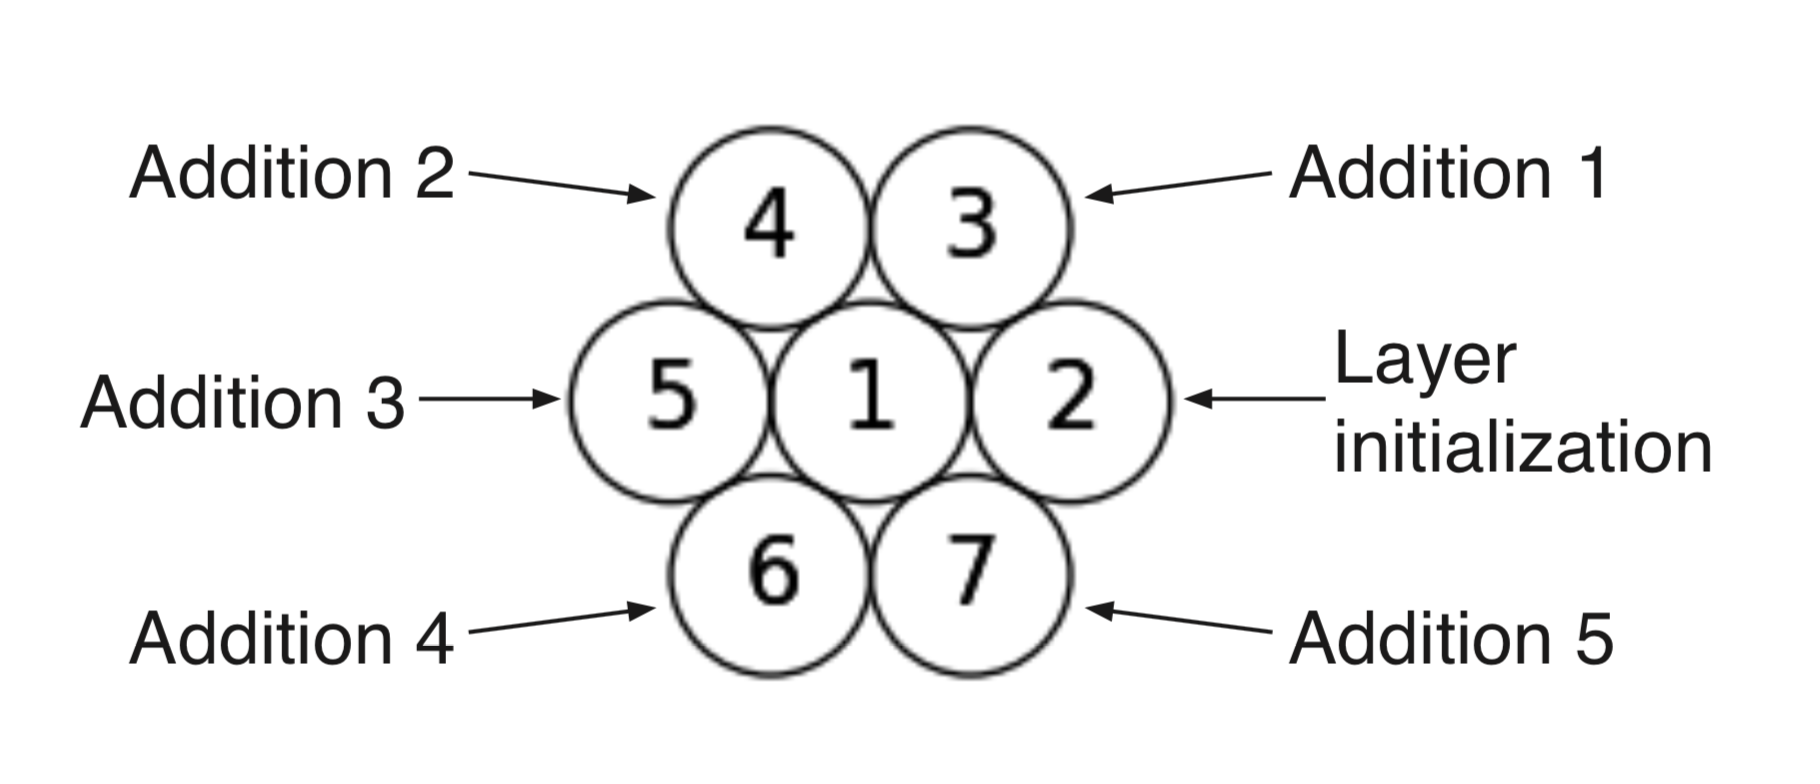
\includegraphics[width=\textwidth]{circles/layer_1}
	\caption{First actuator's layer.}
	\label{fig:appendix:sloan_structure:layer_1}
	\end{subfigure}
	
	\begin{subfigure}{0.70\textwidth}
	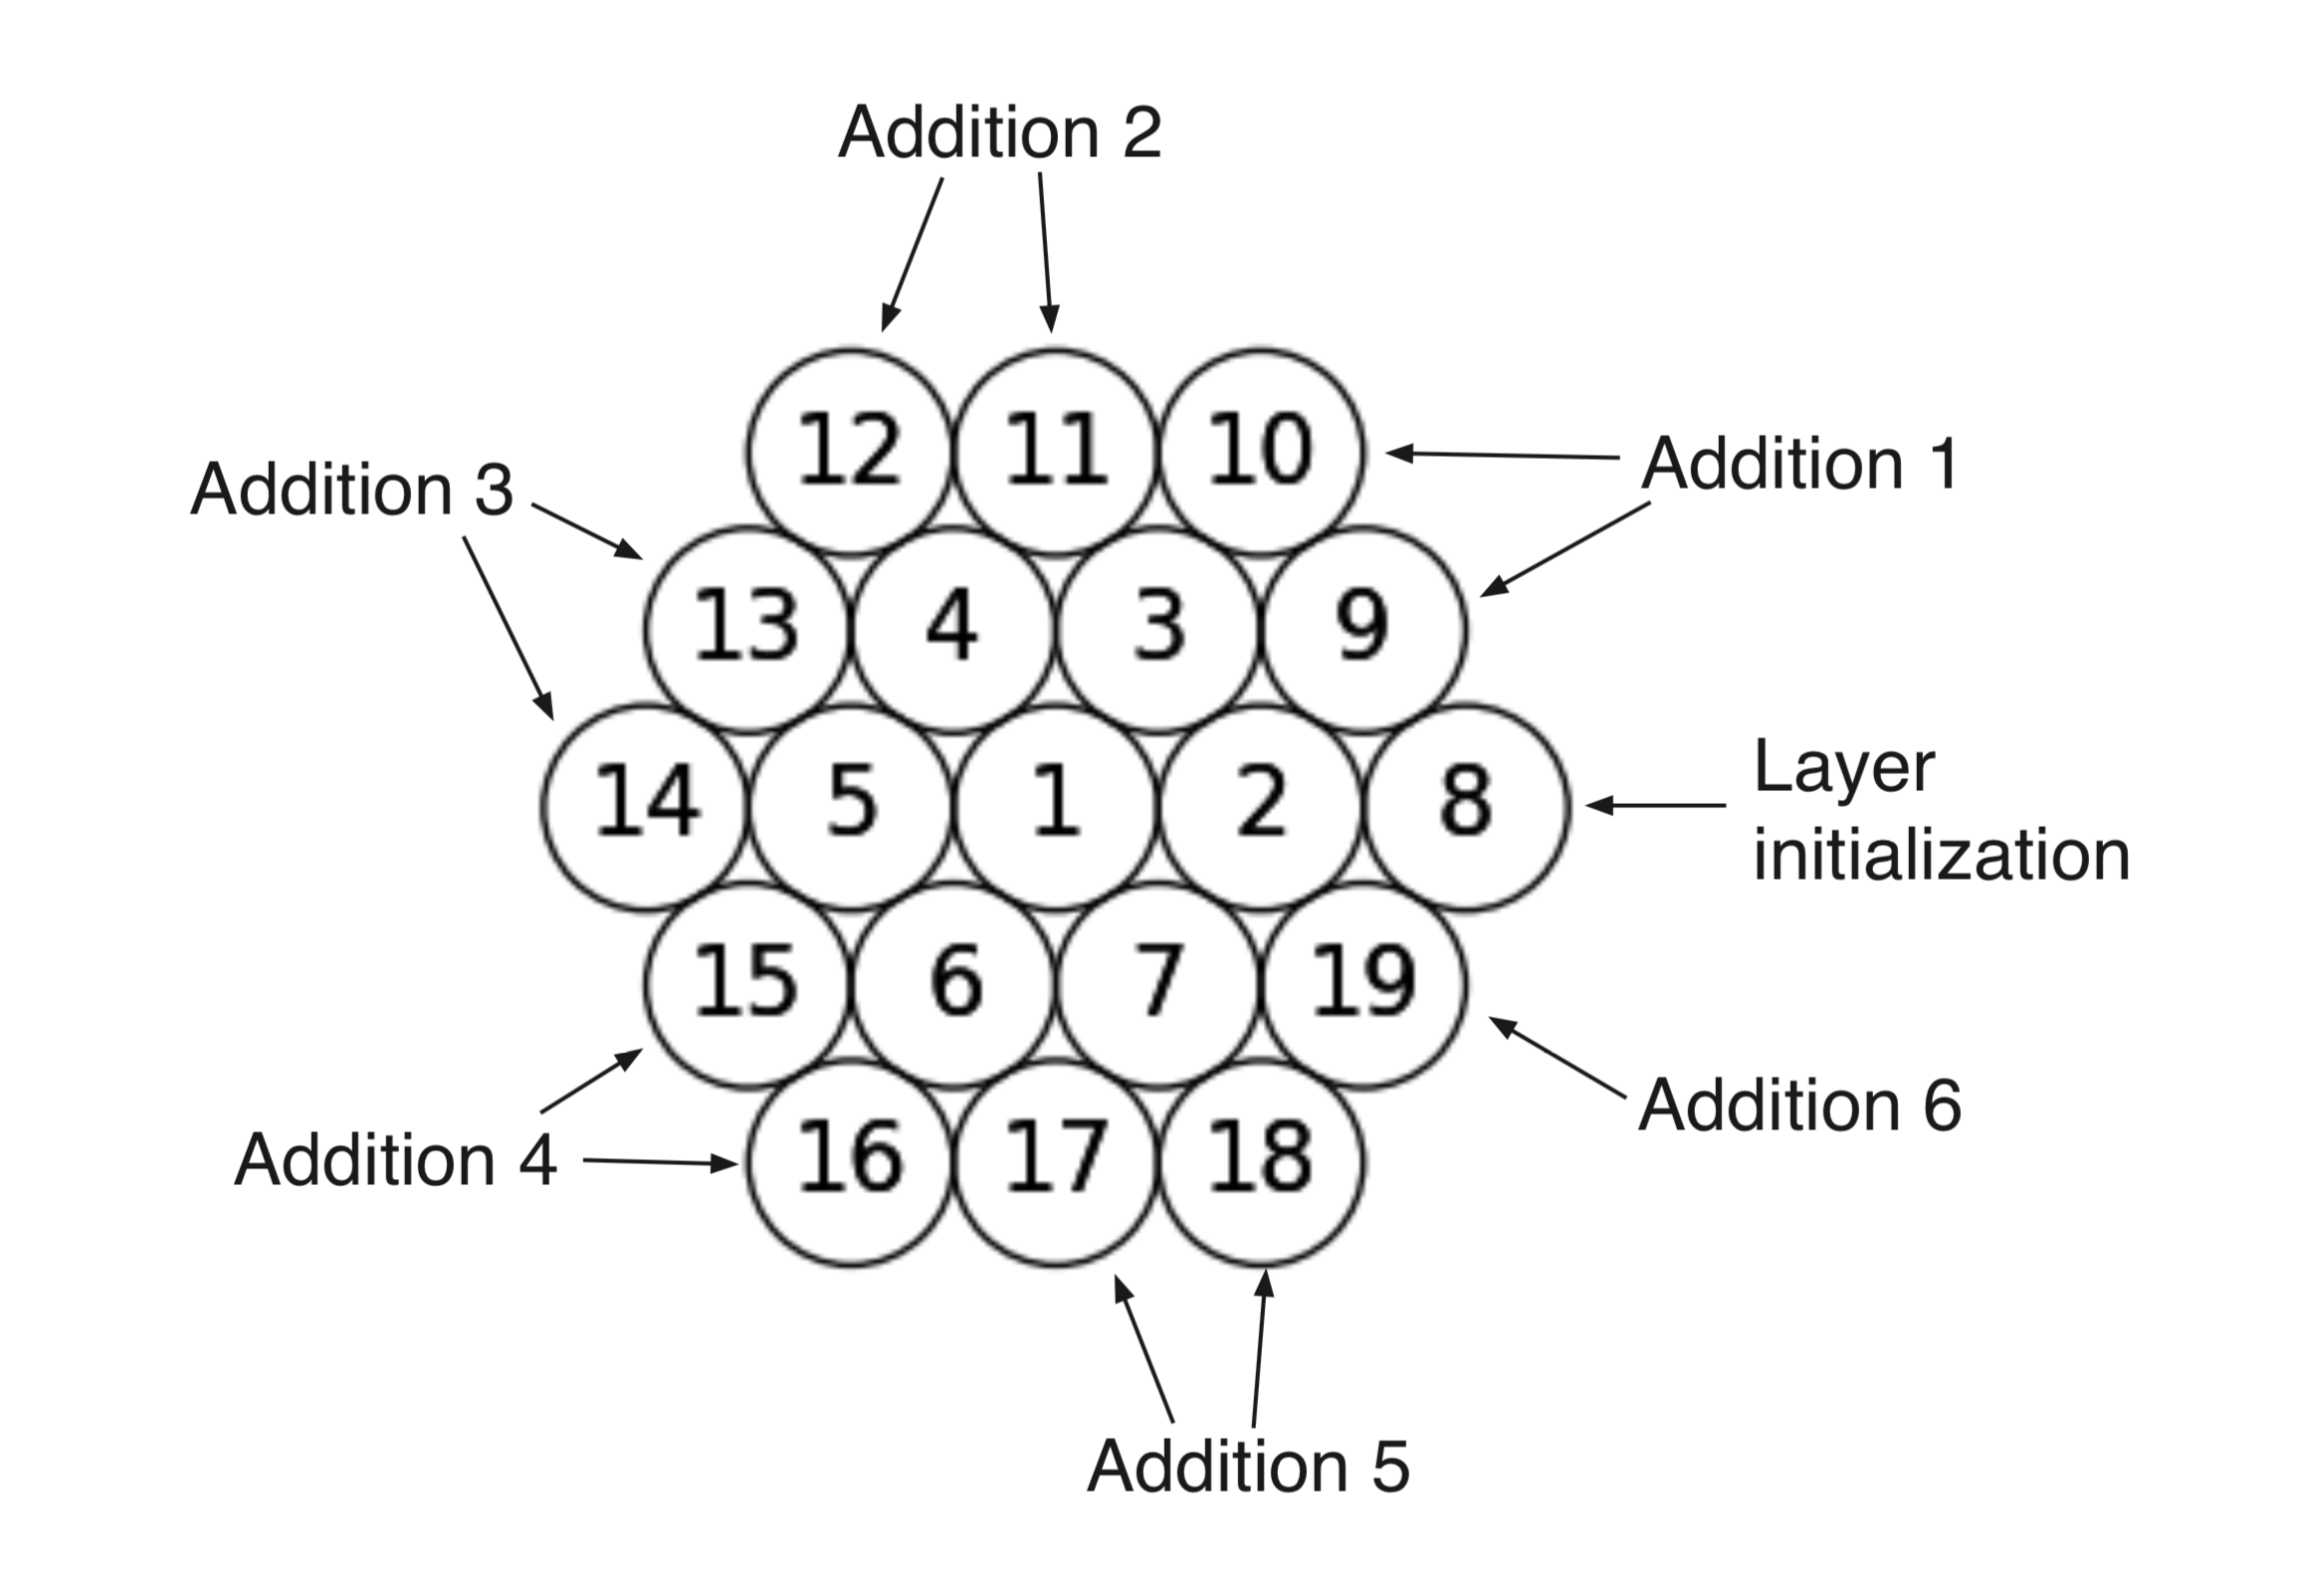
\includegraphics[width=\textwidth]{circles/layer_2}
	\caption{Second actuator's layer.}
	\label{fig:appendix:sloan_structure:layer_2}
	\end{subfigure}
	\caption{Actuators structure explanation: the initialisation creates an actuator at position (0, 0), layer initialisation then creates an actuator on the right, and each addition function creates an actuator close to the last actuator created. $i^{\textrm{th}}$ layer is built by initialising the layer, repeating addition functions 1-5 $i$ times, and finishing by repeating addition function 6 $(i-1)$ times.}
	\label{fig:appendix:sloan_structure}
\end{center}
\end{figure}


\begin{figure}[h]
\begin{center}
	\scriptsize{
	\begin{python}
position.append((0, 0))

def initialisation(num_circle):
    position.append((2*R*num_circle, 0))
    return

def addition_1():
    position.append(tuple((map(operator.add, position[(len(position)-1)], (-R, R * 3 ** 0.5)))))
    return

def addition_2():
    position.append(tuple((map(operator.add, position[(len(position)-1)], (-2*R, 0)))))
    return

def addition_3():
    position.append(tuple((map(operator.add, position[(len(position)-1)], (-R, -R * 3 ** 0.5)))))
    return

def addition_4():
    position.append(tuple((map(operator.add, position[(len(position)-1)], (R, - R * 3 ** 0.5)))))
    return

def addition_5():
    position.append(tuple((map(operator.add, position[(len(position)-1)], (2*R, 0)))))
    return

def addition_6():
    position.append(tuple((map(operator.add, position[(len(position)-1)], (R, R * 3 ** 0.5)))))
    return

def repeat_function(num_circle, function):
    for _ in range(num_circle):function()
    return

def layer_prod(layer):
    initialisation(layer)
    repeat_function(layer, addition_1)
    repeat_function(layer, addition_2)
    repeat_function(layer, addition_3)
    repeat_function(layer, addition_4)
    repeat_function(layer, addition_5)
    repeat_function((layer - 1), addition_6)
    return
	\end{python}
	}
	\caption{Code generating the hexagonal structure shown Figure \ref{fig:sloan:arrangement}. The first line creates the actuator at position (0, 0) (see Figure \ref{fig:appendix:sloan_structure:initialization}). Effects of functions initialisation and addition 1 to 6 are shown on Figure \ref{fig:appendix:sloan_structure:layer_1}. Upper layers (see Figure \ref{fig:appendix:sloan_structure:layer_2}) are built using functions repeat_function and layer_prod.}
	\label{fig:appendix:sloan_structure:code}
\end{center}
\end{figure}


	\clearpage

	\section{Appendix 2: Parameters}

\begin{figure}[h]
\begin{center}
	\scriptsize{
	\begin{python}
INS_POS_LENGTH1 = 8.0
INS_POS_WIDTH1 = 8.0
ALPHA_LIMITS = [-180.0, 180.0]
ALPHA_DEFAULT = 0.0
ALPHA_RPM_LIMITS = [0.73, 2.78]
	\end{python}
	}
	\caption{Former fps_share.py program (code lines 124-128).}
	\label{fig:appendix:parameters_former_fps}
\end{center}
\end{figure}

\begin{figure}[h]
\begin{center}
	\scriptsize{
	\begin{python}
# zone where the positioner is affected by the repulsive force of other positioners
STATUS_OFF_ZONE_INFLUENCE = 3.5
STATUS_ON_ZONE_INFLUENCE = 7.5

LIMITE_FOR_NOISE = 0.08

CSTE_FORCE=6.2
	\end{python}
	}
	\caption{Former pa_dnf.py program (code lines 138-144).}
	\label{fig:appendix:parameters_former_pa_dnf}
\end{center}
\end{figure}


\begin{figure}[h]
\begin{center}
	\scriptsize{
	\begin{python}
sim_length = 210
dt = 0.25
max_speed_alpha = 2*math.pi*2.78/60
min_speed_alpha = 2*math.pi*0.73/60
max_speed_beta = 2*math.pi*3.75/60
min_speed_beta = 2*math.pi*0.98/60
	\end{python}
	}
	\caption{Former path_generator.py program (code lines 39-44).}
	\label{fig:appendix:parameters_former_path}
\end{center}
\end{figure}


\begin{figure}[h]
\begin{center}
	\scriptsize{
	\begin{python}
# PARAMETERS FILE

# Simulation constants
sim_length = 250
dt = 0.25
max_speed_alpha = 2*3.141592653*2.78/60
min_speed_alpha = 2*3.141592653*0.73/60
max_speed_beta = 2*3.141592653*3.75/60 
min_speed_beta = 2*3.141592653*0.98/60

# Dimensions 
INS_POS_LENGTH1 = 7.4
INS_POS_WIDTH1 = 8.0
	\end{python}
	}
	\caption{parameters.txt file.}
	\label{}
\end{center}
\end{figure}


\begin{figure}[h]
\begin{center}
	\scriptsize{
	\begin{python}
import numpy as np

parameters = open('parameters.txt', 'r')
parameters = parameters.read().split()

def look_for(parameter):
    for i in range(0, len(parameters)):
        if parameters[i] == parameter:
            parameter = eval(parameters[i+2])
            break
        else:
            continue

    return parameter

sim_length = look_for('sim_length')
dt = look_for('dt')

max_speed_alpha = look_for('max_speed_alpha')
min_speed_alpha = look_for('min_speed_alpha')
max_speed_beta = look_for('max_speed_beta')
min_speed_beta = look_for('min_speed_beta')
	\end{python}
	}
	\caption{parameters.py program. This program opens the parameters.txt file, and look for parameters by their names using the function look_for (the name inside the function must be exactly the same). When the parameter is found, the function returns the value after the equal sign.}
	\label{}
\end{center}
\end{figure}


\begin{figure}[h]
\begin{center}
	\scriptsize{
	\begin{python}
INS_POS_LENGTH1 = param.INS_POS_LENGTH1
INS_POS_WIDTH1 = param.INS_POS_WIDTH1
ALPHA_LIMITS = [param.ALPHA_TRAVEL_MIN, param.ALPHA_TRAVEL_MAX]
ALPHA_DEFAULT = param.ALPHA_DEFAULT
ALPHA_RPM_LIMITS = [param.ALPHA_RPM_MIN, param.ALPHA_RPM_MAX]
	\end{python}
	}
	\caption{New fps_share.py program.}
	\label{}
\end{center}
\end{figure}


\begin{figure}[h]
\begin{center}
	\scriptsize{
	\begin{python}
# zone where the positioner is affected by the repulsive force of other positioners
STATUS_OFF_ZONE_INFLUENCE = param.STATUS_OFF_ZONE_INFLUENCE
STATUS_ON_ZONE_INFLUENCE = param.STATUS_ON_ZONE_INFLUENCE
LIMITE_FOR_NOISE = param.LIMITE_FOR_NOISE 
CSTE_FORCE = param.CSTE_FORCE
	\end{python}
	}
	\caption{New pa_dnf.py program.}
	\label{}
\end{center}
\end{figure}


\begin{figure}[h]
\begin{center}
	\scriptsize{
	\begin{python}
sim_length = param.sim_length
dt = param.dt
max_speed_alpha = param.max_speed_alpha
min_speed_alpha = param.min_speed_alpha
max_speed_beta = param.max_speed_beta
min_speed_beta = param.min_speed_beta
	\end{python}
	}
	\caption{New path_generator.py program.}
	\label{}
\end{center}
\end{figure}
	\clearpage

	\section{Appendix 3: $\textrm{Set_target}$ update}

\begin{figure}[h]
\begin{center}
	\scriptsize{
	\begin{python}
# Determine the local (wrt positioner centre) coordinates for the
# target.
self.x_fibre_local = self.x_fibre_focal - self.x_centre_focal
self.y_fibre_local = self.y_fibre_focal - self.y_centre_focal
(self.r_fibre_local, self.theta_fibre_local) = util.cartesian_to_polar(self.x_fibre_local, self.y_fibre_local)

if fiber == 1:
	(self.r_fibre_local, self.theta_fibre_local) = (self.r_fibre_local + param.R_CORRECTION_IR, self.theta_fibre_local + param.THETA_CORRECTION_IR)
elif fiber == 0:
	(self.r_fibre_local, self.theta_fibre_local) = (self.r_fibre_local + param.R_CORRECTION_VISIBLE, self.theta_fibre_local + param.THETA_CORRECTION_VISIBLE)
elif fiber == -- 1:
	(self.r_fibre_local, self.theta_fibre_local) = (self.r_fibre_local + param.R_CORRECTION_CALIBRATION, self.theta_fibre_local + param.THETA_CORRECTION_CALIBRATION)
	\end{python}
	}
	\caption{Code modifying the position targeted by the actuator, as function of the fiber used.}
	\label{fig:appendix:set_target:position}
\end{center}
\end{figure}

\begin{figure}[h]
\begin{center}
	\scriptsize{
	\begin{python}
positioner_IR = False
positioner_fiducial = False
positioner_empty = False

for item in circles_test.IR:
	if positioner == item:
		positioner_IR = True

for item in circles_test.fiducial:
	if positioner == item:
		positioner_fiducial = True

for item in circles_test.empty:
	if positioner == item:
		positioner_empty = True

if fiber == 1 and positioner_IR == False:
	return False

if positioner_fiducial == True:
	return False

if positioner_empty == True:
	return False
	\end{python}
	}
	\caption{Code ensuring that Empty and Fiducial can not be set on any target, and that only IR actuator can be set on target desired to be surveyed with an IR fiber.}
	\label{fig:appendix:set_target:attribution}
\end{center}
\end{figure}
	\clearpage
	
	\section{Appendix 4: Software architecture}

\begin{figure}[h]
\begin{center}
	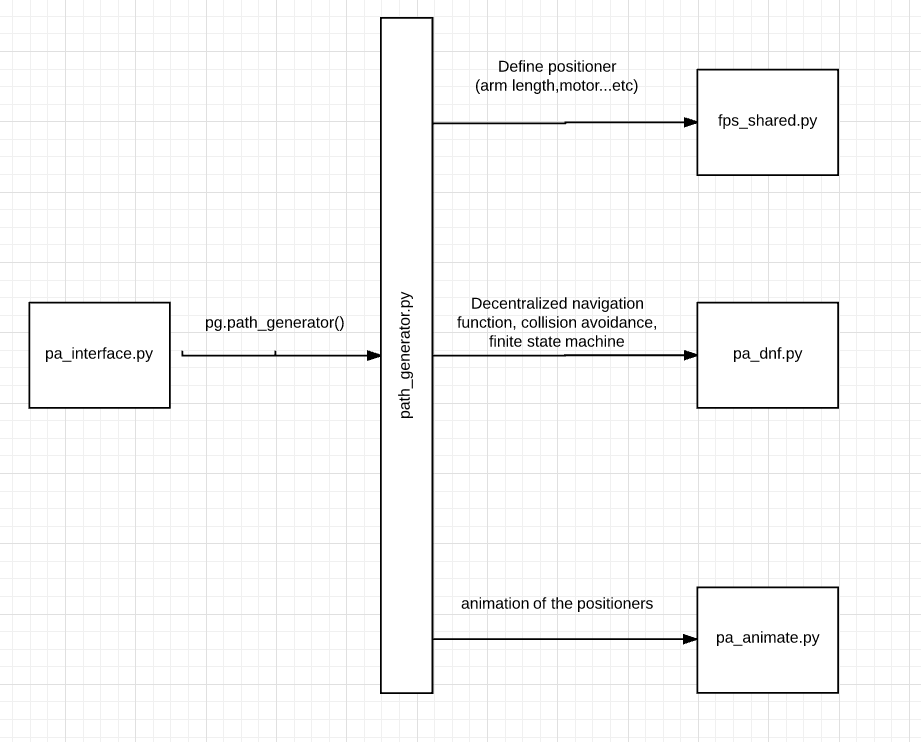
\includegraphics[width=\textwidth]{appendix/former_architecture.png}
	\caption{Former software's architecture.}
	\label{fig:appendix:former_architecture}
\end{center}
\end{figure}

\begin{sidewaysfigure}[h]
\begin{center}
	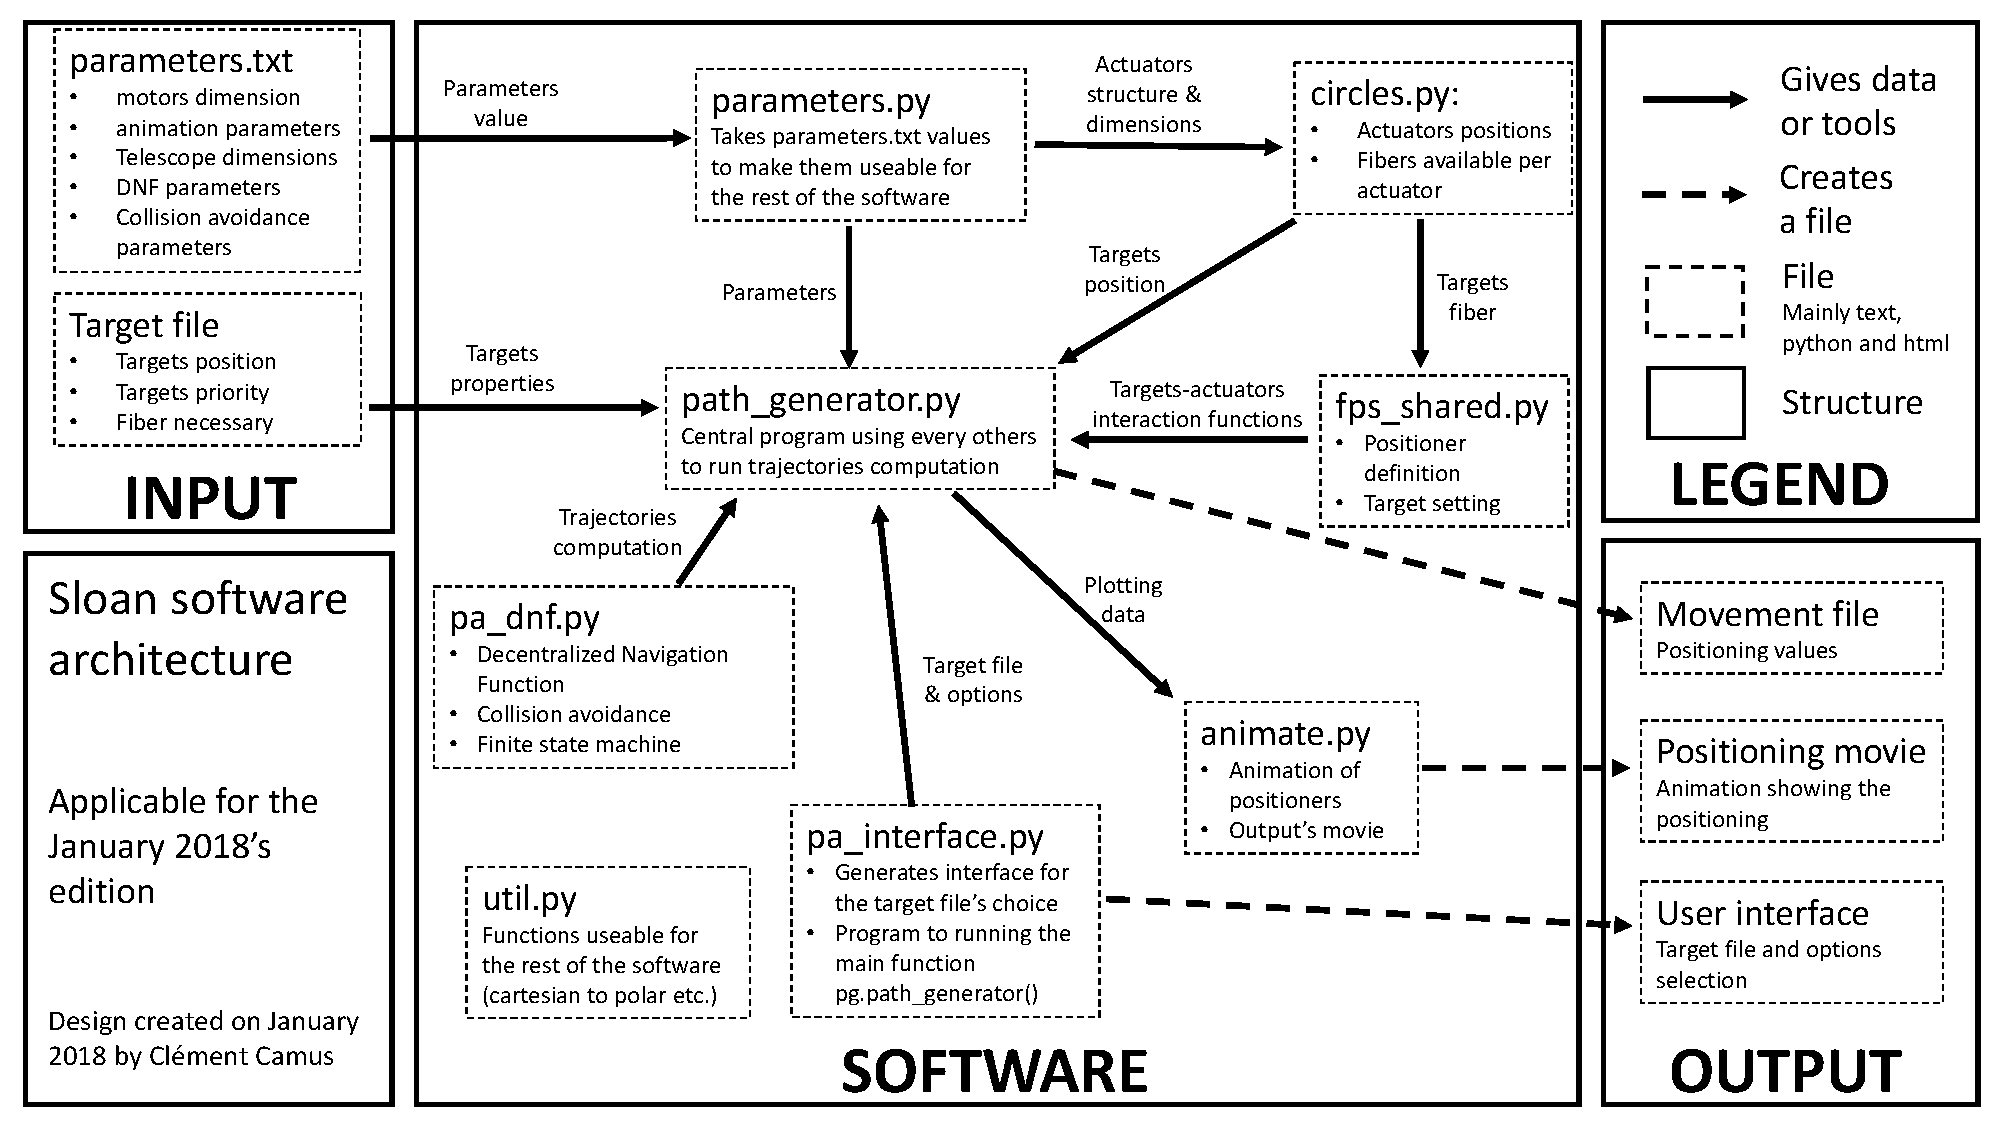
\includegraphics[width=\textwidth]{appendix/new_architecture.pdf}
	\caption{New software architecture.}
	\label{fig:appendix:new_architecture}
\end{center}
\end{sidewaysfigure}

%\begin{figure}[h]
%\begin{center}
%	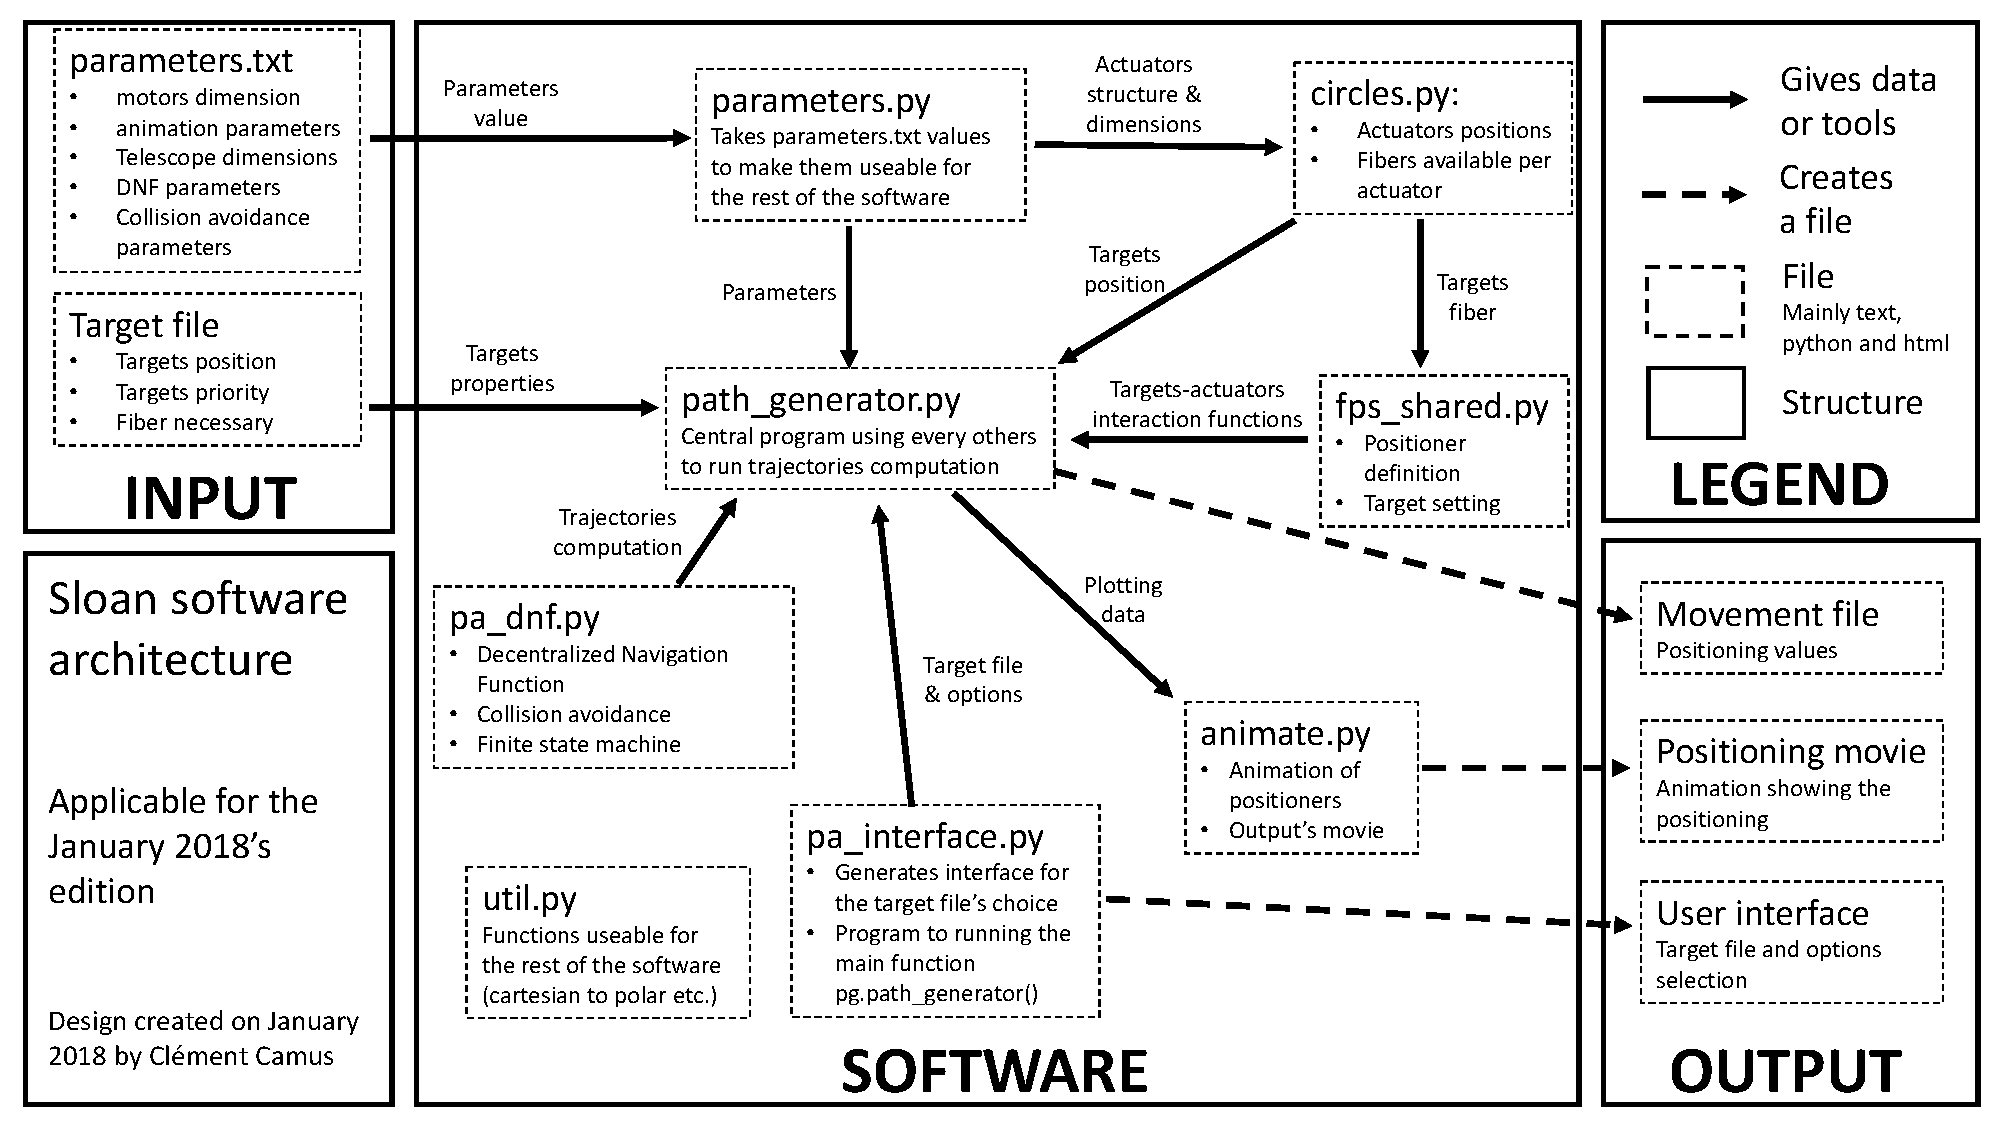
\includegraphics[width=\textwidth]{appendix/new_architecture.pdf}
%	\caption{New software's architecture.}
%	\label{fig:appendix:new_architecture}
%\end{center}
%\end{figure}

	\clearpage

	\section{Appendix 5: Visualisation}

\begin{figure}[h]
\begin{center}
	\scriptsize{
	\begin{python}
    for i, line in enumerate(fr2):
        x1, x2, x3, x4, x5, x6, x7, x8 = map(float, line.split())
        color_target = ''
        if x8 == 1: color_target = 'orange'
        elif x8 == 0: color_target = 'red'
        elif x8 == -1: color_target = 'pink'

        targetcircle = plt.Circle(util.polar_to_cartesian(x3,x4), radius=1, color=color_target, fill=True)
        subfig.add_patch(targetcircle)
	\end{python}
	}
	\caption{Code assigning a color to each targets on the animation, depending on the fiber required for the survey.}
	\label{fig:appendix:visualisation}
\end{center}
\end{figure}
	\clearpage
	
	%\begin{figure}[h]
\begin{center}
	\begin{subfigure}{0.49\textwidth}
		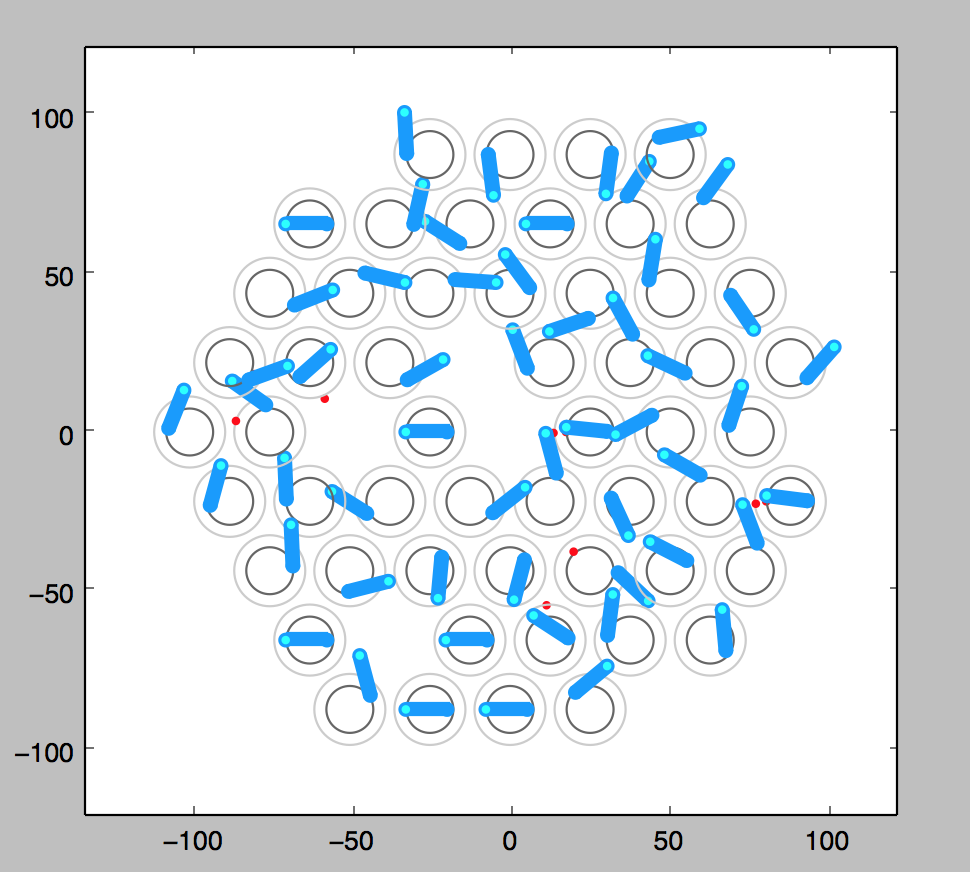
\includegraphics[width=0.9\textwidth]{set_target/sans_correction.png}
		\caption{Résultats pour 60 positionneurs, sans la correction.}
		\label{fig:correction:normal}
	\end{subfigure}
	\begin{subfigure}{0.49\textwidth}
		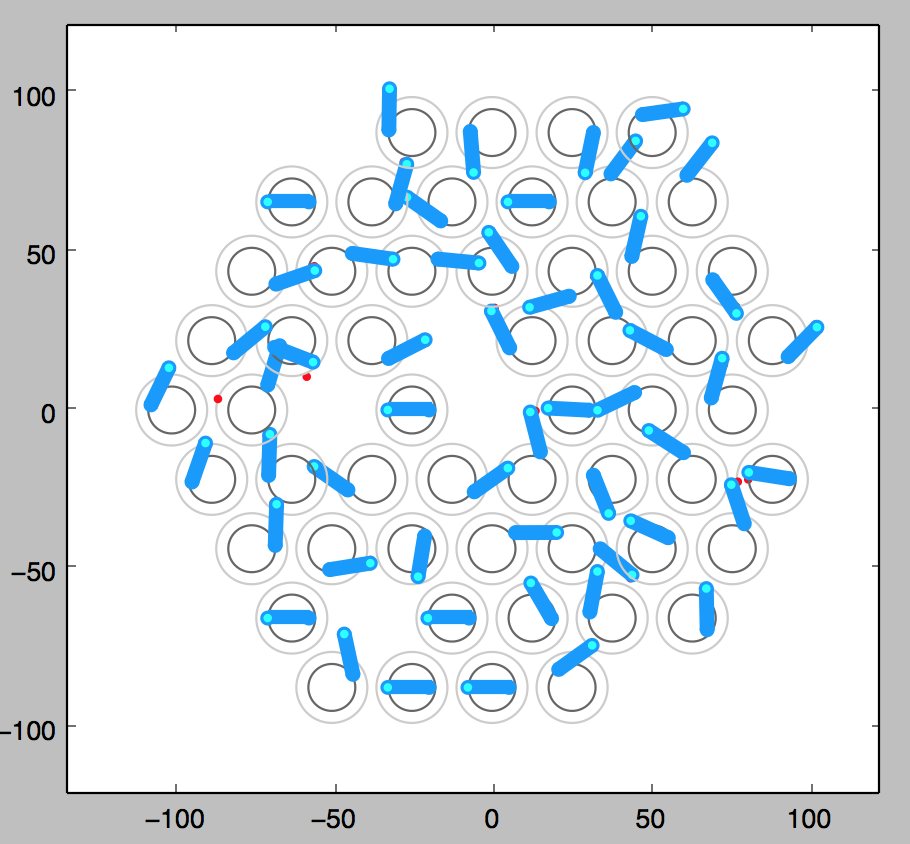
\includegraphics[width=0.9\textwidth]{set_target/correction.png}
		\caption{Résultats pour 60 positionneurs, avec la correction du système.}
		\label{fig:correction:normal}
	\end{subfigure}
	
	\begin{subfigure}{0.49\textwidth}
		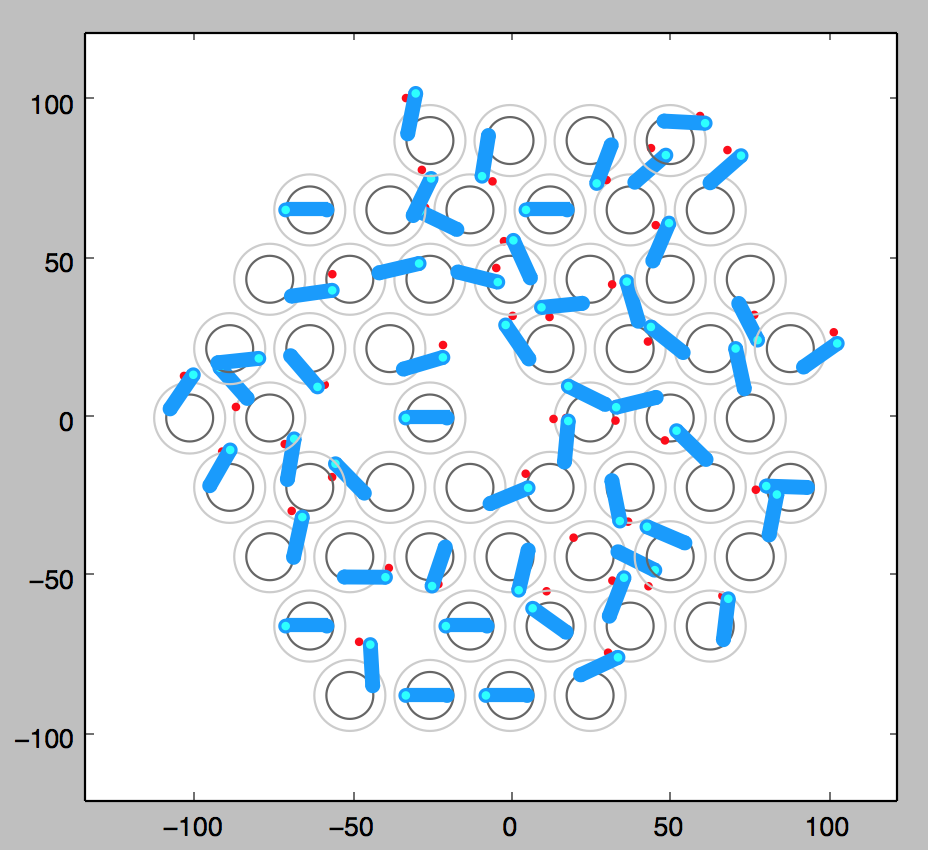
\includegraphics[width=0.9\textwidth]{set_target/correction_x4.png}
		\caption{Résultats pour 60 positionneurs, avec la correction du système multiplié par un facteur 4.}
		\label{fig:correction:normal}
	\end{subfigure}
	\begin{subfigure}{0.49\textwidth}
		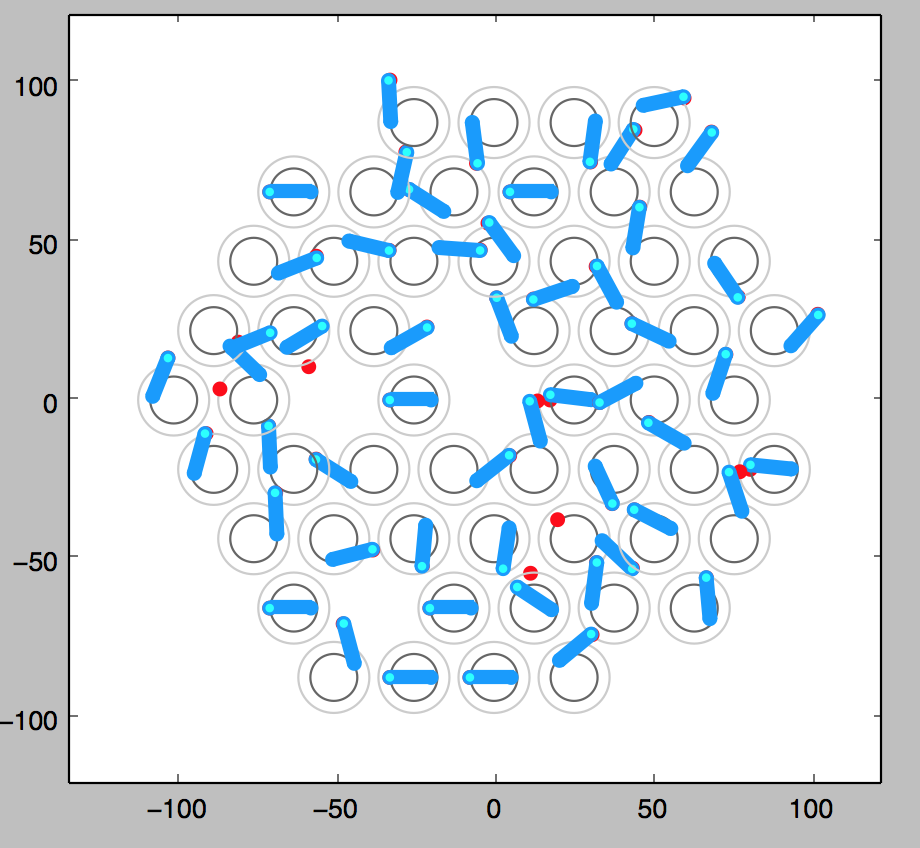
\includegraphics[width=0.9\textwidth]{set_target/sans_correction_r2.png}
		\caption{Résultats pour 60 positionneurs, sans la correction, en élargissant les rayons des targets d'un facteur 2.}
		\label{fig:correction:normal}
	\end{subfigure}
	
	\begin{subfigure}{0.49\textwidth}
		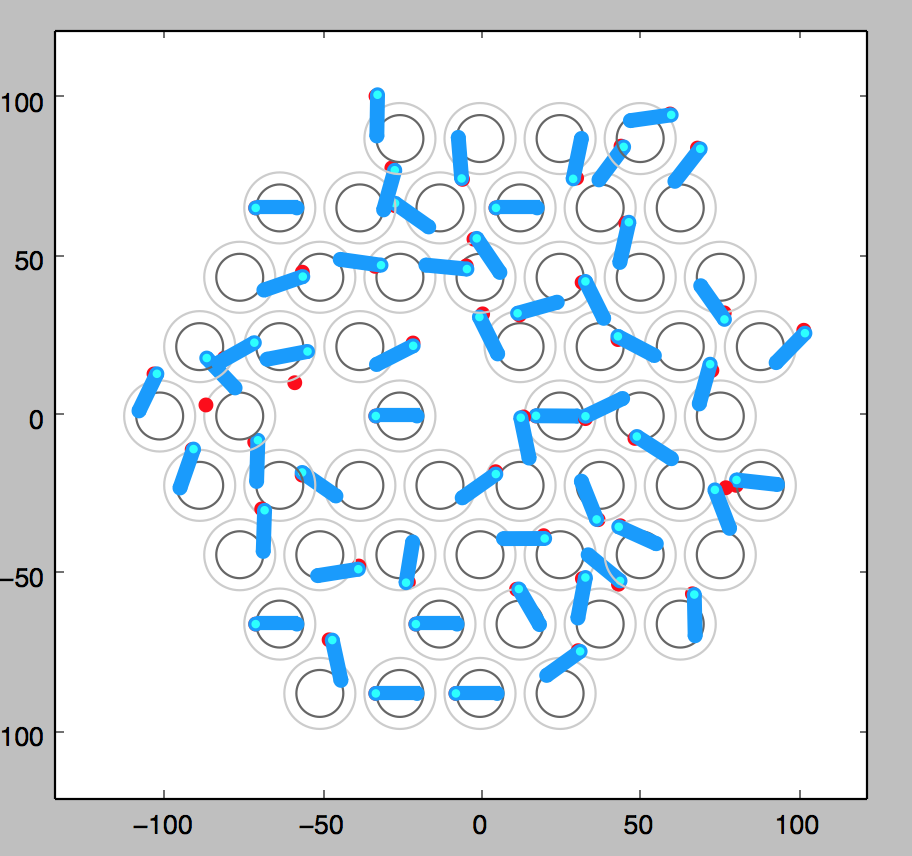
\includegraphics[width=0.9\textwidth]{set_target/correction_r2.png}
		\caption{Résultats pour 60 positionneurs, avec la correction du système, en élargissant les rayons des targets d'un facteur 2.}
		\label{fig:correction:normal}
	\end{subfigure}
	\begin{subfigure}{0.49\textwidth}
		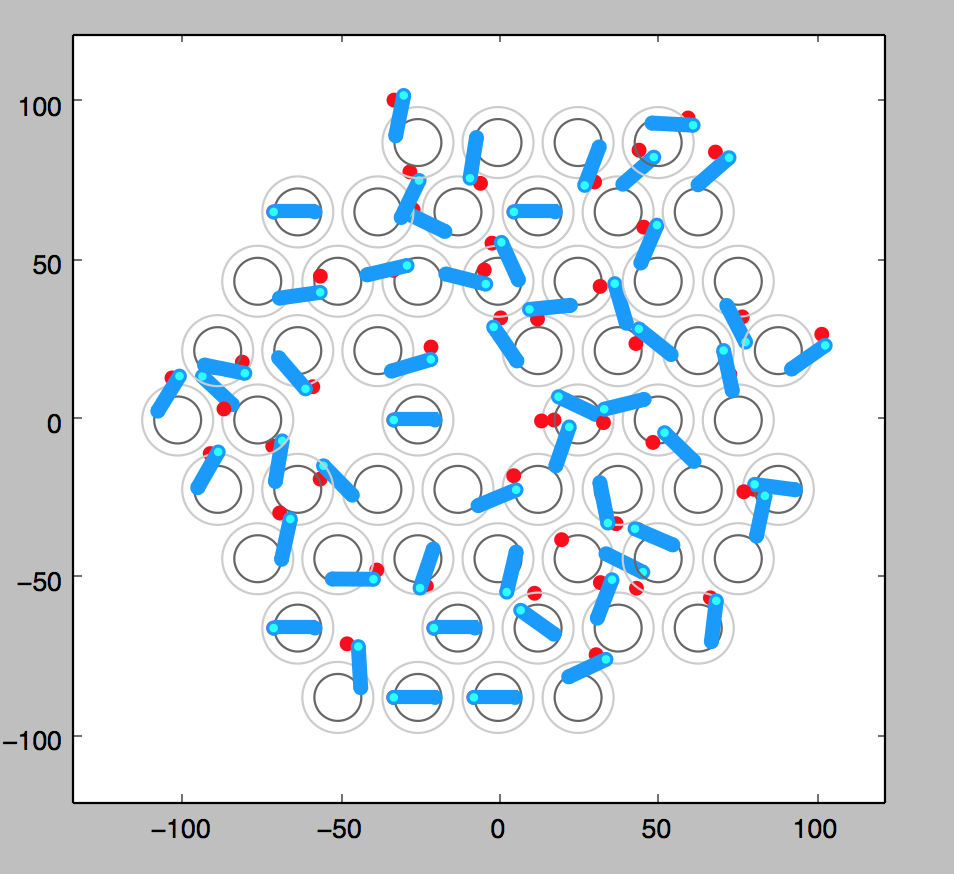
\includegraphics[width=0.9\textwidth]{set_target/correction_x4_r2.png}
		\caption{Résultats pour 60 positionneurs, avec la correction du système multiplié par un facteur 4, en élargissant les rayons des targets d'un facteur 2.}
		\label{fig:correction:normal}
	\end{subfigure}
\end{center}
\end{figure}
	%\clearpage
	
	

	
\end{document}